\subsection{Cycle GANs}
\begin{frame}{}
    \LARGE GAN Variant: \\[1.5ex] \textbf{Cycle GANs}
\end{frame}


\begin{frame}[allowframebreaks]{Cycle GANs}

\begin{itemize}
    \item Unpaired Image-to-Image Translation using Cycle-Consistent Adversarial Networks, Efros, ICC7 2017
    
\end{itemize}
\begin{figure}
    \centering
    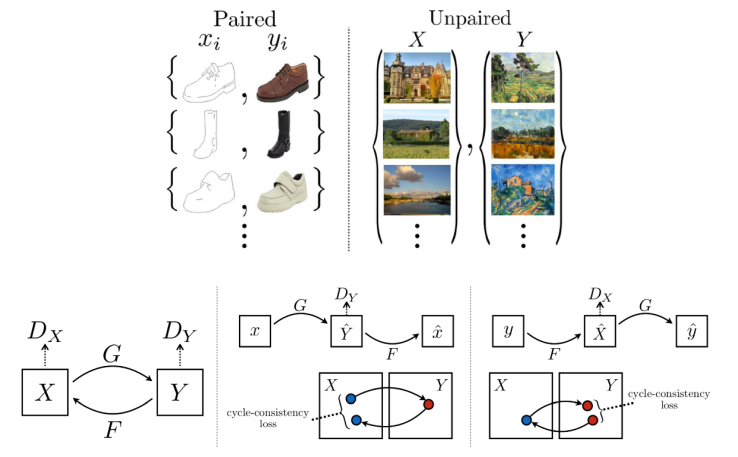
\includegraphics[height=0.7\textheight, width=\textwidth, keepaspectratio]{images/gan/cycle_gan_1.png}
\end{figure}
\framebreak
\textbf{Cycle Consistency}

\begin{itemize}
    \item \textbf{Cycle Consistency Loss:} Ensures that translating an image to the target domain and back yields the original image.
    \item For $x \in X$: $x \rightarrow G(x) = y \rightarrow F(y) \approx x$
    \item \textbf{Mathematically:}
    \[
        \mathcal{L}_{cyc}(G, F) = \mathbb{E}_{x \sim p_{data}(x)} \left[ \| F(G(x)) - x \|_1 \right] + \mathbb{E}_{y \sim p_{data}(y)} \left[ \| G(F(y)) - y \|_1 \right]
    \]
\end{itemize}

\framebreak
\textbf{Total Loss}

\begin{itemize}
    \item \textbf{Adversarial Loss:} Makes generated images indistinguishable from real images.
    \item \textbf{Cycle Consistency Loss:} Enforces reversibility of translation.
    \item \textbf{(Optional) Identity Loss:} Preserves color or structure.
    \item \textbf{Total Loss:}
    \[
        \mathcal{L}_{total} = \mathcal{L}_{GAN}(G, D_Y, X, Y) + \mathcal{L}_{GAN}(F, D_X, Y, X) + \lambda \mathcal{L}_{cyc}(G, F) + \gamma \mathcal{L}_{identity}
    \]
\end{itemize}
\framebreak
$$C_{horse \rightarrow zebra} = horse \rightarrow G_{horse \rightarrow zebra} \rightarrow \hat{zebra} \rightarrow [D_{zebra}, G_{zebra \rightarrow horse}] \rightarrow \hat{horse}$$
\begin{figure}
    \centering
    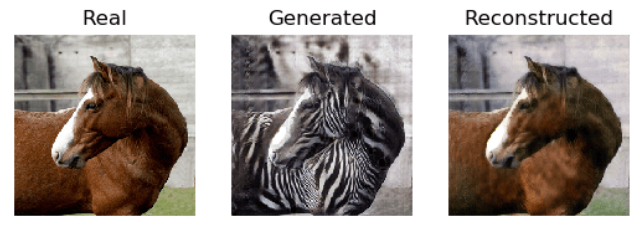
\includegraphics[height=0.7\textheight, width=\textwidth, keepaspectratio]{images/gan/cycle_gan_2.png}
\end{figure}

\framebreak
$$C_{zebra \rightarrow horse} = zebra \rightarrow G_{zebra \rightarrow horse} \rightarrow \hat{horse} \rightarrow [D_{horse}, G_{horse \rightarrow zebra}] \rightarrow \hat{zebra}$$
\begin{figure}
    \centering
    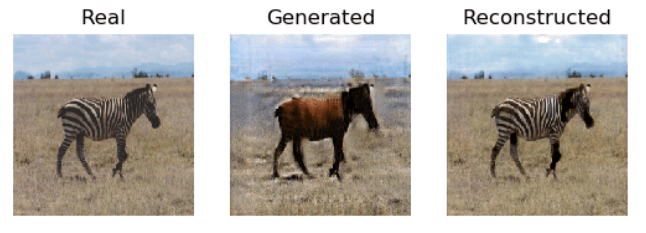
\includegraphics[height=0.7\textheight, width=\textwidth, keepaspectratio]{images/gan/cycle_gan_3.png}
\end{figure}

\framebreak
\begin{figure}
    \centering
    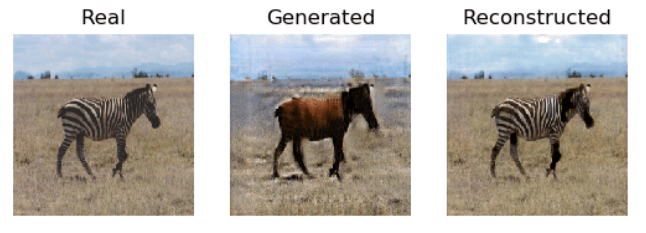
\includegraphics[height=0.7\textheight, width=\textwidth, keepaspectratio]{images/gan/cycle_gan_3.png}
\end{figure}

\framebreak
\begin{figure}
    \centering
    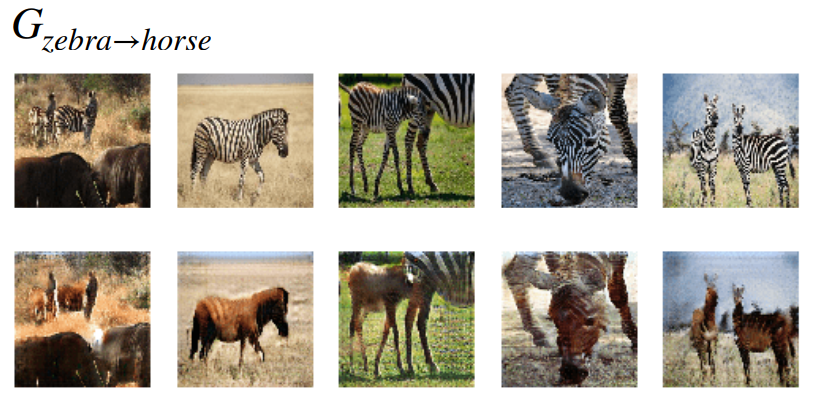
\includegraphics[height=0.9\textheight, width=\textwidth, keepaspectratio]{images/gan/cycle_gan_4.png}
\end{figure}

\framebreak
\begin{figure}
    \centering
    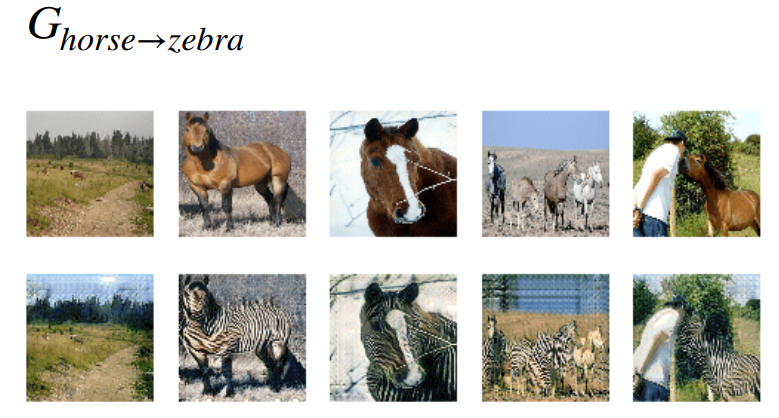
\includegraphics[height=0.9\textheight, width=\textwidth, keepaspectratio]{images/gan/cycle_gan_5.png}
\end{figure}

\framebreak
\begin{figure}
    \centering
    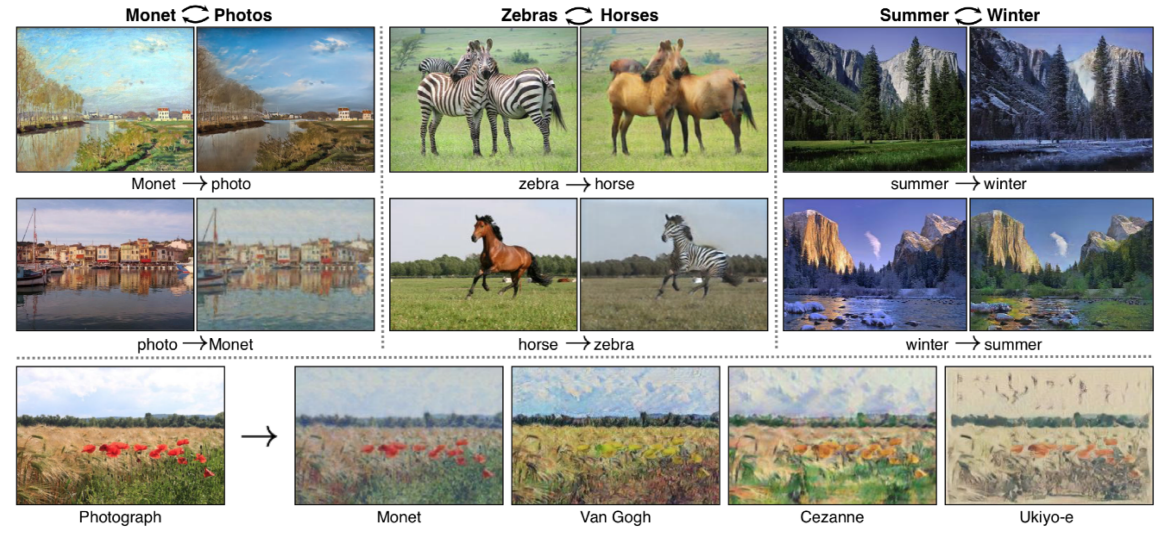
\includegraphics[height=0.9\textheight, width=\textwidth, keepaspectratio]{images/gan/cycle_gan_6.png}
    \caption*{Image to Image translation with Cycle GANs}
\end{figure}
\end{frame}